%%%%%%%%%%%%%%%%%%%%%%%%%%%%%%%%%%%%%%%%%%%%%%%%%%%%%%%%%%%%%%%%%%%%%%%%%%%%%%%
\section{Introduction}
\label{sec:intro}
%%%%%%%%%%%%%%%%%%%%%%%%%%%%%%%%%%%%%%%%%%%%%%%%%%%%%%%%%%%%%%%%%%%%%%%%%%%%%%%
\acs{CERN}'s
Large Hadron Collider~\cite{LHC2008}, know as the \acs{LHC} for short,
is one of the crowning achievements of humankind's quest for knowledge of
our Universe.
%
Arguably one of the largest, most complicated machines ever built,
it smashes together particles at huge energies in a
twenty-seven-kilometre long, colder-than-space underground ring to probe
how matter works at the most fundamental level we can imagine.
It has successfully found, at long last, the particle that we believe gives
massive particles mass -- the celebrated
Higgs boson~\cite{CMS2012a,ATLAS2012c}
for which Peter Higgs
and
François Englert
won the Nobel Prize for Physics in 2013.

The trouble is, it hasn't found anything else -- yet!

%
\begin{figure}[htbp]
  \centering
  \includegraphics[width=0.9\textwidth]{assets/images/lhc-aerial/LHC-PHO-1986-002.jpg}
  \caption[An aerial view of Geneva showing the location of the LHC]
  {\label{fig:lsstartistimpr}An aerial view of Geneva showing the location of \acs{CERN}'s \acf{LHC}. Image credit: \href{http://cds.cern.ch/record/841527}{J.-L. Caron/CERN 1986-2016}; please contact them regarding licensing/re-use of this image.}
\end{figure}
%

Well, that's not fair. The four largest experiments located at the
four Interaction Points (IPs) on
the \ac{LHC}'s ring -- \acs{ALICE}~\cite{ALICE2008},
\acs{ATLAS}~\cite{ATLAS2008},
\acs{CMS}~\cite{CMS2008},
and
\acs{LHCb}~\cite{LHCb2008} -- have made many discoveries that have furthered
our understanding of physics of the very, very small.
%
All of these, however, pretty much fit into our current best understanding
of how matter and forces work -- known as
the Standard Model of particle physics -- of which the Higgs boson was
the missing piece.
%
In that sense, the \acs{LHC} has been a huge success,
and the thousands of physicists and engineers who made it work -- and
the public who funded it -- should be immensely proud of its achievements.

%
\begin{figure}[htbp]
  \centering
  \includegraphics[width=0.7\textwidth]{assets/images/standard-model/standard-model-cern_WEB.jpg}
  \caption[The Standard Model of particle physics]
  {\label{fig:standardmodel}The Standard Model of particle physics, now %
completed with the Higgs boson. %
Image credit: \href{https://cds.cern.ch/journal/CERNBulletin/2012/35/News Articles/1473657}{D. Galbraith/C. Burgard/CERN 2012}; %
please contact them regarding licensing/re-use of this image.}
\end{figure}
%

What we'd like to do, however, is go beyond the Standard Model and
answer questions like:
\begin{itemize}
\item How did particles interact at the very beginning of the Universe?
\item Can we unite all of the forces into one Grand Unified Theory?
\item What is Dark Matter, the ``missing fifth'' of the Universe?
\item Why is there more matter than antimatter?
\item How can we describe gravity at very small scales?
\item How many dimensions does our Universe have?
\item Why do neutrinos have mass?
\end{itemize}
We can't answer these questions with the Standard Model.
More research is required, and as the \acs{LHC}~\cite{LHC2008} collects
more data at the record-breaking 13 \ac{TeV},
\acs{ALICE}~\cite{ALICE2008},
\acs{ATLAS}~\cite{ATLAS2008},
\acs{CMS}~\cite{CMS2008},
and
\acs{LHCb}~\cite{LHCb2008}
will do their best to answer them.
There is, however, another fundamental question about our Universe
that pre-dates even the Standard Model.

\newpage

%=============================================================================
\subsection{A lack of symmetry: where’s the magnetic charge?}
\label{sec:magcharge}
%=============================================================================
When James Clerk-Maxwell unified the electric and magnetic forces into one
``electromagnetic'' force in 1865~\cite{Maxwell1865},
his famous four equations (shown in Figure~\ref{fig:maxwellseqs})
lacked a certain symmetry.

% Maxwell's equations
\begin{figure}[htbp]
  \centering
\begin{eqnarray}
\label{eq:1} \divvec{\electricfield} & = & \highlight{4 \pi \electricchargedensity} \\ [10pt]
\label{eq:2} \divvec{\magneticfield} & = & 0\\ [10pt]
\label{eq:3} - \curlvec{\electricfield} & = & \myfrac{1}{\speedoflight} \, \timediff{\magneticfield}\\ [10pt]
\label{eq:4}   \curlvec{\magneticfield} & = & \myfrac{1}{\speedoflight} \, \timediff{\electricfield} + \highlight{\myfrac{4 \pi}{\speedoflight} \, \electriccurrentdensity}
\end{eqnarray}
  \caption[Maxwell's equations of electromagnetism]
  {\label{fig:maxwellseqs}Maxwell's equations of electromagnetism~\cite{Maxwell1865} with the electric charge and current density terms highlighted (shaded boxes). Note that these are expressed in Gaussian units (not SI) for simplicity.}
\end{figure}

%
Don't worry about exactly what these all mean for the moment.
The terms in the shaded boxes are what we're interested in:
these represent electric charge (static and moving).
Electric charge is a property of matter that experiences
interactions via the electromagnetic force.
Electric charge can be positive or negative; like charges repel
each other while opposite charges attract.
%
The question that physicists have asked ever since -- starting
with Marie Skłodowska Curie's husband Pierre~\cite{Curie1894} -- is
is why there is no equivalent term for magnetic charge and current,
which would make the equations look like those shown in
Figure~\ref{fig:maxwellseqsmagcharge}.

% Maxwell's equations with magnetic charge.
\begin{figure}[htbp]
  \centering
\begin{eqnarray}
\label{eq:1m} \divvec{\electricfield} & = & 4 \pi \electricchargedensity\\ [10pt]
\label{eq:2m} \divvec{\magneticfield} & = & 4 \pi \magneticchargedensity\\ [10pt]
\label{eq:3m} - \curlvec{\electricfield} & = & \myfrac{1}{\speedoflight} \, \timediff{\magneticfield} + \myfrac{4 \pi}{\speedoflight} \, \magneticcurrentdensity\\ [10pt]
\label{eq:4m}   \curlvec{\magneticfield} & = & \myfrac{1}{\speedoflight} \, \timediff{\electricfield} + \myfrac{4 \pi}{\speedoflight} \, \electriccurrentdensity
\end{eqnarray}
  \caption[Maxwell's equations of electromagnetism with magnetic charge]
  {\label{fig:maxwellseqsmagcharge}Maxwell's equations of electromagnetism with additional terms representing magnetic charge and current density, as shown on the cover of the MoEDAL Technical Design Report~\cite{MoEDAL2009}. Note that these are expressed in Gaussian units (not SI) for simplicity.}
\end{figure}

Much nicer, no? In practical terms, what these different equations would
mean that some matter could have ``magnetic charge''.
Magnetic charges would exert a force -- via a magnetic field -- on
other matter with magnetic charge in just the same way as matter
with electric charge.
The problem is that we never have never seen isolated magnetic charge.
The magnets we see always have a North and a South pole
(the equivalent of positive and negative charge) -- and so are dipoles.
\term{Magnetic monopoles} -- matter with just a North or a
South pole (see Figure~\ref{fig:dipolemonopole}) -- have not yet
been seen in an experiment.

%
\begin{figure}[htbp]
  \centering
  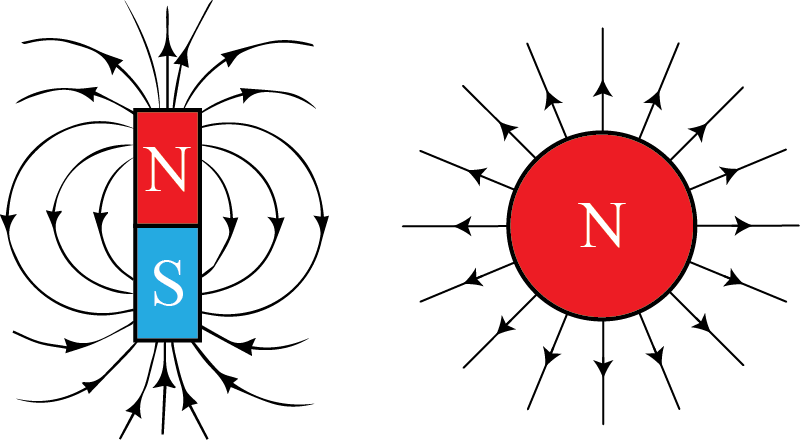
\includegraphics[width=0.7\textwidth]{assets/images/dipole-vs-monopole/dipole-vs-monopole.png}
  \caption[A magnetic dipole and monopole]
  {\label{fig:dipolemonopole}A magnetic dipole with North and South poles (left); a magnetic monopole, North pole only (right).  Image credit: \href{http://researchinschools.org}{Institute for Research in Schools}.}
\end{figure}
%

%=============================================================================
\subsection{The MoEDAL experiment}
\label{sec:moedalintro}
%=============================================================================
The \acf{MoEDAL}~\cite{MoEDAL2009}
%The Monopole and Exotics Detector at the LHC~\cite{MoEDAL2009}
is the latest and greatest in a long line of experiments which aims to
finally find evidence for the existence of magnetic monopoles.
%
It is designed to hunt for monopoles created in particle collisions
at the LHC using methods tailored to the strange properties of monopoles
and other highly-ionising particles.
As such it complements the searches for \ac{BSM} physics as performed by
the other LHC experiments,
providing another exciting way we can try to answer fundamental questions 
about our Universe.

%
\begin{figure}[htbp]
  \centering
  \includegraphics[width=0.9\textwidth]{assets/images/moedal-photo/MoEDAL-IMG-001.jpg}
  \caption[The MoEDAL experiment at CERN]
  {\label{fig:moedalphoto}The MoEDAL experiment at CERN.
Image credit: \href{http://moedal.web.cern.ch/}{The MoEDAL Collaboration/CERN};
please contact them regarding licensing/re-use of this image.}
\end{figure}
%

As we'll see,
one of these special techniques requires human input.
Many experiments can automate their searches for new physics using computer
programs because they use electronic readouts and are, generally speaking,
looking for well-understood particles.
%
The MoEDAL detector systems -- and the particles they are
looking for -- are very different,
and so require the human brain's enormous capability for image processing,
decision-making, and all-round ability to spot things that are ``odd''.
Which is where you come in -- MoEDAL needs your help!


%=============================================================================
\subsection{Overview of this guide}
\label{sec:overview}
%=============================================================================
Section~\ref{sec:theory} discusses the theory behind magnetic monopoles,
and presents a number of ideas that motivate the search for them.
The searches that have been carried out to-date are presented in
Section~\ref{sec:search}.
The MoEDAL experiment is described in more detail in
Section~\ref{sec:exp}, and finally the ways the reader may get involved
with MoEDAL is described in Section~\ref{sec:getinvolved}.
